\documentclass{beamer}

\usepackage[utf8]{inputenc}
\usepackage{graphicx}
\usepackage{hyperref}
\usepackage{tikz}
\usetikzlibrary{shapes.geometric, positioning, arrows.meta, calc}

% Theme selection
\usetheme{Madrid}
\usecolortheme{default}

\title{PharmAssist System Flow}
\subtitle{Chronological Journey of an AI Voice Interaction}
\author{Mihir}
\institute{M.Tech Major Project Presentation}
\date{\today}

\begin{document}

% Title Slide
\begin{frame}
    \titlepage
\end{frame}

% 1. Problem Statement
\begin{frame}{1. Problem Statement}
    \begin{itemize}
        \item \textbf{Operational Bottleneck:} Highly trained pharmacists are constantly interrupted by trivial, repetitive phone calls (stock, pricing, hours).
        \item \textbf{IVR Failures:} Traditional Interactive Voice Response systems ("Press 1 for stock") use rigid decision trees and lack Natural Language Understanding.
        \item \textbf{The Solution:} PharmAssist uses a GenAI-powered conversational agent to handle these queries naturally and autonomously.
    \end{itemize}
    \vspace{0.5cm}
    \centering
    % Placeholder for System Architecture Diagram
    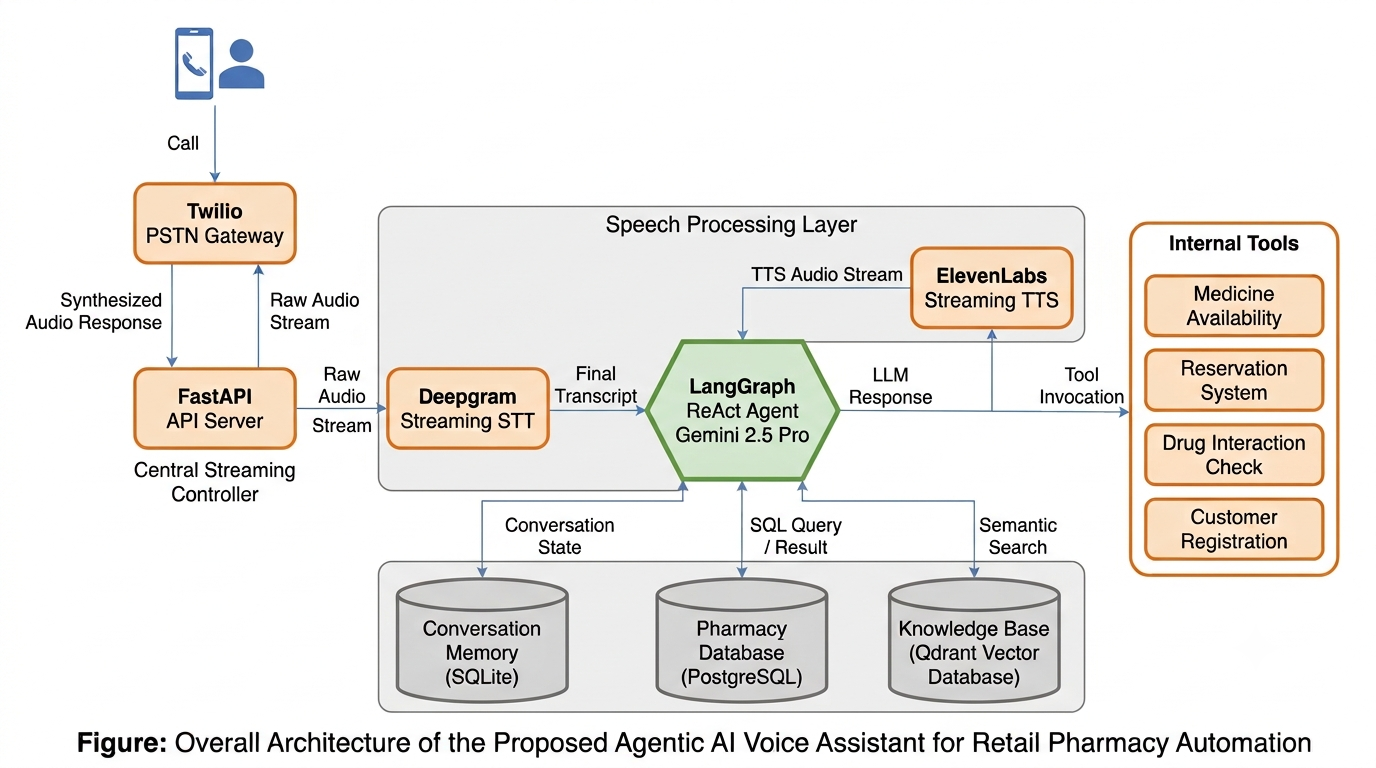
\includegraphics[width=0.7\textwidth]{archietecture.png} % Replace with actual filename if different
\end{frame}

% 2. Twilio Configuration
\begin{frame}{2. Twilio Configuration}
    \begin{itemize}
        \item \textbf{The Bridge:} Twilio intercepts the PSTN (Public Switched Telephone Network) signal when a user calls.
        \item \textbf{WebSockets:} Configured via TwiML to initiate a \texttt{<Stream>} command, opening a continuous, bidirectional WebSocket to our FastAPI server.
        \item \textbf{Audio Format:} Streams raw audio in \textbf{G.711 $\mu$-law format at 8000Hz} for ultra-low latency.
    \end{itemize}
\end{frame}

% 3. Deepgram Configuration
\begin{frame}{3. Deepgram Configuration}
    \begin{itemize}
        \item \textbf{Streaming API:} The server opens a persistent WebSocket connection to Deepgram for instant Speech-to-Text transcription.
        \item \textbf{Voice Activity Detection (VAD):} Deepgram monitors the audio for exactly \textbf{500 milliseconds of absolute silence}.
        \item \textbf{Turn-Taking:} Once the silence threshold is met, it emits a \texttt{speech\_final} flag, instantly letting the system know the user finished speaking.
    \end{itemize}
\end{frame}

% 4. Agent Workflow
\begin{frame}{4. Agent Workflow}
    \begin{itemize}
        \item \textbf{The Core Engine:} LangGraph ReAct (Reasoning and Acting) Agent, powered by \textbf{Google's Gemini 2.5 Pro}.
        \item \textbf{Cyclical Logic (ReAct Loop):}
        \begin{itemize}
            \item \textbf{Observe:} Analyzes user intent and conversation history.
            \item \textbf{Reason:} Evaluates if it needs to fetch external data (like checking inventory).
            \item \textbf{Act:} Generates structured JSON to trigger a Python tool, ingests the result, and loops back to reason until ready to reply.
        \end{itemize}
    \end{itemize}
\end{frame}

% 5. Tables Available & All Tools (Part 1 - Tables)
\begin{frame}{5. Tables Available}
    \begin{itemize}
        \item \textbf{Database Architecture:} Uses a secure PostgreSQL/SQLite database with exactly 3 core tables to prevent AI hallucinations.
        \item \textbf{The 3 Tables and their Exact Fields:}
        \begin{itemize}
            \item \texttt{medicines}: (\texttt{id, name, generic\_name, strength, manufacturer, price, stock, created\_at, updated\_at})
            \item \texttt{customers}: (\texttt{id, name, phone, created\_at})
            \item \texttt{orders}: (\texttt{id, customer\_id, medicine\_id, quantity, status, reserved\_at})
        \end{itemize}
    \end{itemize}
\end{frame}

% 5. Tables Available & All Tools (Part 1.5 - Images)
\begin{frame}{Admin Portal - Access \& Customers}
    \centering
    % Placeholder for Login Screenshot
    \includegraphics[width=0.45\textwidth]{login.png}
    \hfill
    % Placeholder for Customers Screenshot
    \includegraphics[width=0.45\textwidth]{customers.png}
\end{frame}

% 5. Tables Available & All Tools (Part 2 - Tools)
\begin{frame}{5. All Tools \& Functionality}
    \begin{itemize}
        \item \textbf{Customer Tools:}
        \begin{itemize}
            \item \texttt{register\_customer}: Registers using name and 10-digit phone.
            \item \texttt{get\_customer}: Retrieves profile using phone number.
            \item \texttt{update\_customer}: Modifies existing customer's name.
        \end{itemize}
        \item \textbf{Medicine Tools:}
        \begin{itemize}
            \item \texttt{search\_medicine}: Pattern-match search by brand/generic name.
            \item \texttt{check\_stock}: Returns exact units available.
            \item \texttt{list\_available\_medicines}: Complete list of drugs in stock > 0.
        \end{itemize}
        \item \textbf{Order Tools:}
        \begin{itemize}
            \item \texttt{reserve\_medicine}: Deducts stock using atomic database row-locking.
            \item \texttt{cancel\_order}: Restores stock count to inventory.
            \item \texttt{get\_order\_status}: Retrieves fulfillment state.
        \end{itemize}
    \end{itemize}
\end{frame}

% 5.5. First-Time Customer Order Flow Diagram
\begin{frame}{Order Flow: First-Time Customer}
    \centering
    \resizebox{\textwidth}{!}{
    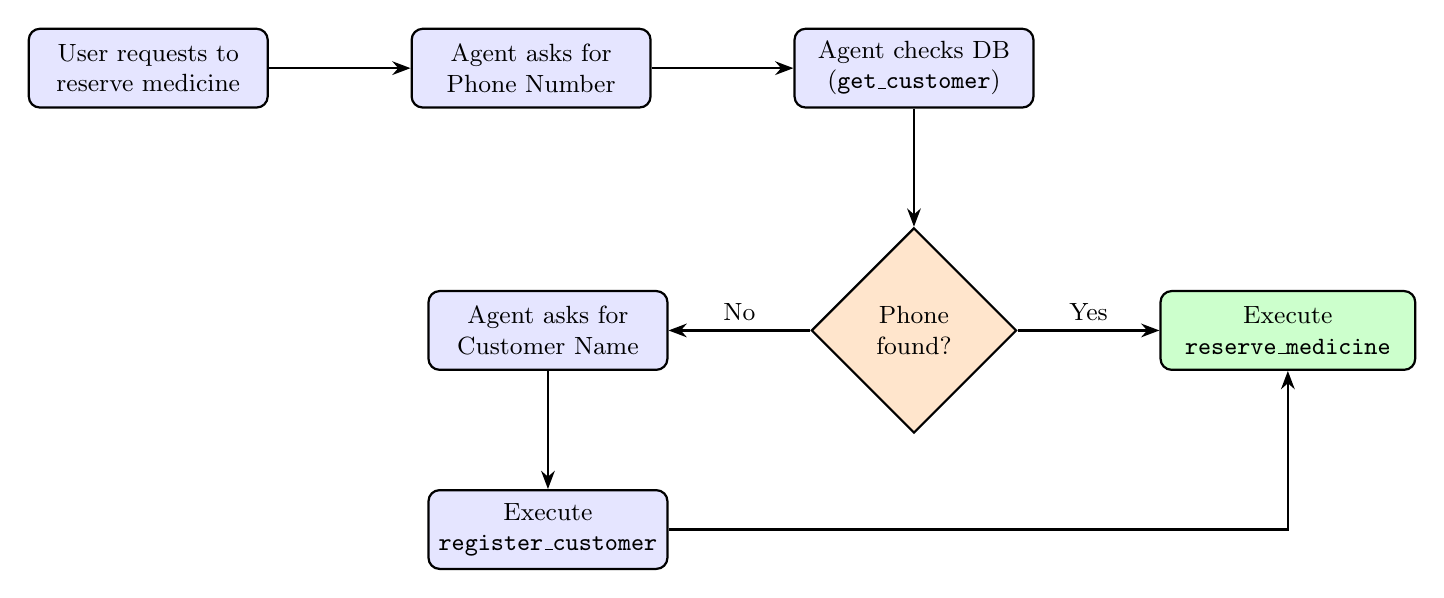
\begin{tikzpicture}[
        node distance=1.5cm and 1.8cm,
        >=Stealth,
        every node/.style={font=\small},
        process/.style={rectangle, rounded corners, draw, thick, fill=blue!10, text width=2.8cm, align=center, minimum height=1cm},
        decision/.style={diamond, draw, thick, fill=orange!20, text width=2cm, align=center, inner sep=0pt, minimum height=2cm},
        endpoint/.style={rectangle, rounded corners, draw, thick, fill=green!20, text width=3cm, align=center, minimum height=1cm}
    ]
        % Nodes
        \node[process] (start) {User requests to reserve medicine};
        \node[process, right=of start] (askPhone) {Agent asks for \\ Phone Number};
        \node[process, right=of askPhone] (dbCheck) {Agent checks DB (\texttt{get\_customer})};
        \node[decision, below=of dbCheck] (isFound) {Phone \\ found?};
        
        \node[process, left=of isFound] (askName) {Agent asks for \\ Customer Name};
        \node[process, below=of askName] (register) {Execute \\ \texttt{register\_customer}};
        
        \node[endpoint, right=of isFound] (placeOrder) {Execute \\ \texttt{reserve\_medicine}};
        
        % Arrows
        \draw[->, thick] (start) -- (askPhone);
        \draw[->, thick] (askPhone) -- (dbCheck);
        \draw[->, thick] (dbCheck) -- (isFound);
        
        \draw[->, thick] (isFound) -- node[above] {No} (askName);
        \draw[->, thick] (askName) -- (register);
        \draw[->, thick] (register) -| (placeOrder);
        
        \draw[->, thick] (isFound) -- node[above] {Yes} (placeOrder);
        
    \end{tikzpicture}
    }
\end{frame}

% 6. RAG Architecture for Medicine Details
\begin{frame}{6. RAG Architecture for Medicine Details}
    \begin{itemize}
        \item \textbf{The Goal:} Safely answer pharmacological questions without hallucinating.
        \item \textbf{Vector Embeddings:} Uses \textbf{gemini-embedding-2} to convert natural language queries to high-dimensional vectors.
        \item \textbf{Custom Vector Store:} Instead of a slow external database, it calculates \textbf{Cosine Similarity} in-memory using \textbf{NumPy arrays} for ultra-low latency.
        \item \textbf{System Prompt Injection:} Injects retrieved medical paragraphs into Gemini's prompt, enforcing factual answers.
    \end{itemize}
    \vspace{0.2cm}
    \centering
    % Placeholder for RAG Diagram
    \includegraphics[width=0.6\textwidth]{rag_flow.png} % Replace with actual RAG diagram filename
\end{frame}

% 7. How Conversation is Preserved
\begin{frame}{7. How Conversation is Preserved}
    \begin{itemize}
        \item \textbf{The Stateless Challenge:} WebSockets naturally forget previous turns.
        \item \textbf{SqliteSaver Checkpointer:} LangGraph assigns a unique Call SID (\texttt{thread\_id}).
        \item \textbf{State Memory:} Agent's memory graph is serialized into a local SQLite database (\texttt{checkpoints.db}) after every step.
        \item \textbf{Instant Rehydration:} When user speaks again, \texttt{thread\_id} instantly rehydrates the state.
    \end{itemize}
    \vspace{0.2cm}
    \centering
    % Placeholder for Conversation Logs Screenshot
    \includegraphics[width=0.6\textwidth]{conversation_logs.png}
\end{frame}

% 8. Browser Chat & Voice Integration
\begin{frame}{8. Browser Chat \& Voice Integration}
    \begin{itemize}
        \item \textbf{Omnichannel Client:} An integrated web client for users who prefer not to call via phone.
        \item \textbf{Text \& Voice Options:} Supports standard typed text chat.
        \item \textbf{Live Microphone Integration:} Streams microphone audio directly to the backend via WebSockets, mirroring the exact Twilio low-latency flow in the browser.
    \end{itemize}
\end{frame}

% 9. ElevenLabs Configuration
\begin{frame}{9. ElevenLabs Configuration}
    \begin{itemize}
        \item \textbf{TTS Synthesis:} The Agent's final textual response is routed via HTTP to ElevenLabs.
        \item \textbf{Voice Cloning:} Generates highly realistic human speech with natural intonation.
        \item \textbf{Zero Latency Transcoding:} API is configured to return audio natively in the \texttt{ulaw\_8000} format.
        \item \textbf{The Output:} The raw audio is instantly piped back into the Twilio (or Browser) WebSocket, allowing the caller to hear the response in under a second.
    \end{itemize}
\end{frame}

% 10. Future Enhancements
\begin{frame}{10. Future Enhancements}
    \begin{itemize}
        \item \textbf{EHR/EMR Integration:} Secure integration with Electronic Health Records for automated prescription verification and processing.
        \item \textbf{Multi-Lingual Support:} Expanding the STT and TTS engines to support regional languages for broader accessibility.
        \item \textbf{Outbound Capabilities:} Automated outbound calls for prescription refill reminders and appointment scheduling.
        \item \textbf{Insurance API Integration:} Real-time fetching of co-pay amounts and insurance coverage verification during the call.
    \end{itemize}
\end{frame}

% End Slide
\begin{frame}
    \centering
    \Huge Thank You! \\
    \vspace{1cm}
    \large
    \textbf{Live Deployment:} Deployed using Railway \\
    \vspace{0.2cm}
    \normalsize
    \href{https://web-production-1a1a.up.railway.app}{https://web-production-1a1a.up.railway.app}
\end{frame}

\end{document}
